\documentclass[letterpaper, 10 pt, conference]{ieeeconf}  % Comment this line out
                                                          % if you need a4paper
%\documentclass[a4paper, 10pt, conference]{ieeeconf}      % Use this line for a4
                                                          % paper

\IEEEoverridecommandlockouts                              % This command is only
                                                          % needed if you want to
                                                          % use the \thanks command
\overrideIEEEmargins
% See the \addtolength command later in the file to balance the column lengths
% on the last page of the document

\usepackage[pdftex]{graphicx}

\title{\LARGE \bf
TODO Name this thing
}

% TODO which style do we use for authors? and do we list all 4 of us here?

%\author{ \parbox{3 in}{\centering Huibert Kwakernaak*
%         \thanks{*Use the $\backslash$thanks command to put information here}\\
%         Faculty of Electrical Engineering, Mathematics and Computer Science\\
%         University of Twente\\
%         7500 AE Enschede, The Netherlands\\
%         {\tt\small h.kwakernaak@autsubmit.com}}
%         \hspace*{ 0.5 in}
%         \parbox{3 in}{ \centering Pradeep Misra**
%         \thanks{**The footnote marks may be inserted manually}\\
%        Department of Electrical Engineering \\
%         Wright State University\\
%         Dayton, OH 45435, USA\\
%         {\tt\small pmisra@cs.wright.edu}}
%}

\author{Huibert Kwakernaak$^{1}$ and Pradeep Misra$^{2}$% <-this % stops a space
% \thanks{$^{1}$H. Kwakernaak is with Faculty of Electrical Engineering, Mathematics and Computer Science,
%         University of Twente, 7500 AE Enschede, The Netherlands
%         {\tt\small h.kwakernaak at papercept.net}}%
% \thanks{$^{2}$P. Misra is with the Department of Electrical Engineering, Wright State University,
%         Dayton, OH 45435, USA
%         {\tt\small p.misra at ieee.org}}%
}

\long\def\commentp#1{{\bf **Peter: #1**}}
\long\def\commentpk#1{{\bf **Piyush: #1**}}
\long\def\commentm#1{{\bf **Mike: #1**}}
\long\def\commentd#1{{\bf **Dustin: #1**}}

\begin{document}

\maketitle
\thispagestyle{empty}
\pagestyle{empty}

%%%%%%%%%%%%%%%%%%%%%%%%%%%%%%%%%%%%%%%%%%%%%%%%%%%%%%%%%%%%%%%%%%%%%%%%%%%%%%%%

\commentd{sounds fine to me, only thing is that we haven't actually focused on
  dynamic re-planning or any kind of overseer yet, although theres nothing
  stopping us from trying that idea again}

\begin{abstract}
Autonomous vehicles have seen great advancements in recent years and such vehicles are now ever closer to being commercially available. The advent of driver-less cars provides opportunities for optimizing traffic in ways not possible before. This paper introduces an open source multi-agent traffic simulator called AORTA, which stands for \textit{Approximately Orchestrated Road Traffic Automata}, and demonstrates its usage for optimizing autonomous traffic at a city-wide scale. AORTA creates scale simulations by generating maps using publicly available road data from \textit{OpenStreetMap} (OSM). Simulations can be set up in the few minutes it takes to export data for the region of interest from OSM. AORTA focuses on interactions between agents by defining \textit{behaviors} for individual vehicles and intersections. These behaviors allow agents to interact with each other as well as with an external \textit{overseer} that is responsible for optimizing traffic flow. Overseers can interact with these agents to allow for dynamic route re-planning to reduce traffic load, optimized intersection navigation, and improved car following. \commentpk{rest devoted to application}
\end{abstract}

%%%%%%%%%%%%%%%%%%%%%%%%%%%%%%%%%%%%%%%%%%%%%%%%%%%%%%%%%%%%%%%%%%%%%%%%%%%%%%%%

\section{INTRODUCTION}
\label{sec:introduction}

% what are our goals with this paper?
% theme: easy simulation in your city, in 2 minutes!
% * demonstrate use of OSM and motivate more data collection
% * present a simulation framework
% * present a pretty naive static planning
% * motivate and demonstrate wards for hierarchial planning (but also reasoning
%    about congestion)
% be sure to emphasize open source!

% contribution: autonomous car / human car sim on EXISTING INFRASTRUCTURE

Autonomous vehicle technology has made tremendous progress in the last decade. In 2004, the farthest distance traveled by a vehicle autonomously in the DARPA Grand Challenge was $11.9km$ \cite{cnnGrandChallenge2004}. By 2007, six of the competing teams completed the $96km$ course set for the DARPA Urban Challenge \cite{spectrumUrbanChallenge2007}. They did so while following the same traffic laws followed by human drivers, navigating along with other moving vehicles, and following correct intersection precedence order. Since then, Google's driver-less cars have clocked more than $250,000km$ on public roads in urban California, USA \cite{tedThrun2011}. In 2010, researchers from the University of Parma successfully completed an autonomous \textit{intercontinental} run from Parma, Italy to Shanghai, China \cite{cnnVislab2010}. The successful completion of all these milestones indicates that autonomous cars are here to stay, and are ever closer to becoming commercially available. 

The arrival of driver-less cars presents a number of challenges that need to addressed in the near term. Road infrastructure needs to be updated to better support autonomous vehicles. A number of legal and safety concerns need to be addressed in the context of driver-less cars. Human drivers need new methodologies to interact with autonomous drivers on public roads. At the same time, driver-less cars provide opportunities of solving traffic problems in ways that were never before possible. For instance, autonomous cars can be quickly diverted to make way for emergency vehicles responding to an accident. Even day-to-day traffic issues such as congestion could potentially be greatly reduced by effective management of traffic flow. This work attempts to address some of these problems.

\commentd{nevada even made autonomous cars legal:
http://www.pcmag.com/article2/0,2817,2400400,00.asp}

\commentd{another example long-term usage: fuel. I went to a talk by
  somebody on the engr side about powermiling and optimizing battery usage}

\commentd{we don't support lane-changing yet, and overseers arent re-implemented
yet either}

This paper introduces an open source multi-agent microscopic traffic simulator called AORTA, which stands for \textit{Approximately Orchestrated Road Traffic Automata}. The AORTA simulator focuses on the interactions between individual vehicles and intersections, both of which act as \textit{agents} in AORTA's framework. Vehicles interact with other vehicles to pass and change lanes, and interact with intersections to decide when to cross them. Researchers developing applications on top of the AORTA simulator define \textit{behaviors} that these agents follow to interact with one another. To optimize traffic flow, external \textit{overseers} can coordinate with these agents to provide recommendations such as route suggestions or intersection signaling policies. An advantage of such an approach is that by assigning human-like behaviors such as the "car following model" \cite{brackstone1999car} to vehicles and traffic signal like policies to intersection, AORTA can just as easily simulate human traffic.

Like any other microscopic traffic simulator, AORTA needs maps to run simulations. We generate our maps using road data available from OpenStreetMap (OSM) \cite{osm}, a Wikipedia like interface for world maps. Researchers using AORTA can export the relevant map area from OSM that is then parsed by AORTA to create scale simulations of the real world. Using real world road data is advantageous for a number of reasons. First, researchers using AORTA for human traffic simulations would find it advantageous to also have the ability to use real-world roads. Second, even as infrastructural changes will be made to the road infrastructure to accommodate driver-less cars, it is reasonable to assume that the \textit{same} road network will still be in use. Third, using real-world data from OSM allows setting up simulations for an area of interest in a matter of minutes, thereby allowing easy transfer of research results to any desired region.

\commentd{The first reason for real world data almost feels too obvious to state
like that}

\commentpk{Needs 1 more para based on final application, and image on the top right, and introduction to the rest of the paper here once we finalize the sections}

% Section 2 will review other traffic simulators. Section 3 will introduce the
% overall architecture of AORTA. Section 4 describes how OSM maps are used.
% Section 5 explains the simulation engine and the properties AORTA posses that
% are useful for general traffic experiments. Section 6 gives some initial
% results from such an experiment, and Section 7 concludes.

%%%%%%%%%%%%%%%%%%%%%%%%%%%%%%%%%%%%%%%%%%%%%%%%%%%%%%%%%%%%%%%%%%%%%%%%%%%%%%%%

\section{RELATED WORK}
\label{sec:related_work}

Computational processing power has made excellent advancements in the last two decades. Parallel computing has proved significant for traffic simulation through the use of Geographic Information System (GIS) software \cite{pursula1999simulation}. Advanced computing techniques have enabled microscopic models of traffic simulation to generate results at a meaningful scale (city-wide or greater). As a result, a number of good micro-simulators have come up in the past decade. We review a number of such simulators in this section along with other relevant work.  

A number of traffic simulators already make use of OSM data. MATSim is one such multi-agent simulator that focuses on performing large-scale simulations in a relatively small amount of time \cite{balmer2009matsim}. Traffic demand is supplied to MATSim in the form of \textit{plans} that an individual may intend to follow in a given day. MATSim aims to iteratively improve these plans though offline computation to maximize traffic throughput. In other words, it helps individuals understand the best way to go about their daily routine to minimize time spent in transit. This goal is somewhat different from that of AORTA, where the demand supplied by individuals is taken as is. Instead, AORTA aims to reduce traffic congestion through interactions with individuals in real-time based on the current demand.

Another popular open source traffic simulator that can use OSM data is SUMO \cite{SUMO2011}, which shares the same goals as AORTA and is fairly similar at a high level. SUMO has been used to study the effect of automated transportation systems, route planning of individual vehicles, as well as dynamically adapting traffic signal policies to increase traffic efficiency. AORTA and SUMO differ in the manner in which intersections are handled. SUMO uses traditional traffic signals, while AORTA adopts a much more general \textit{reservation} system. A reservation tells a car when it is safe to take its desired path through the intersection. Reservations can be alotted to vehicles through more traditional means such as traffic signals or stop-sign based intersection based precedence, or through more efficient methods designed specificaly for autonomous intersection management \cite{JAIR08-dresner}. \commentpk{does this difference seem a bit pedantic?}  

On the other hand, there are a number of simulators that specifically target autonomous traffic systems. One such system is AIM \cite{JAIR08-dresner}, which aims to optimize traffic flow between autonomous vehicles at a given intersection. AIM studies problems at the scale of a single intersection, while AORTA has the potential to apply some of the same research at a city-wide scale to real-world road networks. A few simulators focus on autonomous vehicles with sensors and actuators \cite{figueiredo2009approach}. These simulators are used to ensure that autonomous vehicles are behaving correctly while interacting with other vehicles and infrastructure. On the other hand, AORTA assumes that autonomous vehicles are capable of reasonable driving, and focuses on interactions between agents to optimize traffic flow. 

Autonomous agents have also been used in the past to model human traffic as well. For instance, an approach models human merging and lane changing behavior through the use of autonomous agents interacting with one another \cite{hidas2002modelling}. Another approach attempted to improve traffic congestion for human drivers by using a network of autonomous intersection. These intersections have the ability to interact with one another and execute a dynamic traffic signal policy minimizing overall wait time \cite{manikonda2001autonomous}.

\commentd{and we can do the above too. we talk about how to make the current
  behavior more flawed and humanlike in the agent reactions section.}

\commentpk{I suspect there are still more papers that might be more relevant - we'll definitely have some when we write the application}

% In the realm of applications
% It is also necessary to analyze some other simulators that use GIS data for microscopic traffic simulations, this is because it may be possible to export OSM data so that it can be used by these simulators, though the authors are not aware of such a connection. Incident response has been studied by the following paper (though perhaps only a minor citation as it is an application and does not really compare against AORTA, but it is something we would like to study this as well. \cite{huang2007gis} 

%%%%%%%%%%%%%%%%%%%%%%%%%%%%%%%%%%%%%%%%%%%%%%%%%%%%%%%%%%%%%%%%%%%%%%%%%%%%%%%%

\section{ARCHITECTURE}

{ 
  \begin{center}
    \setlength\fboxsep{0pt}
    \setlength\fboxrule{0.5pt}
    \fbox{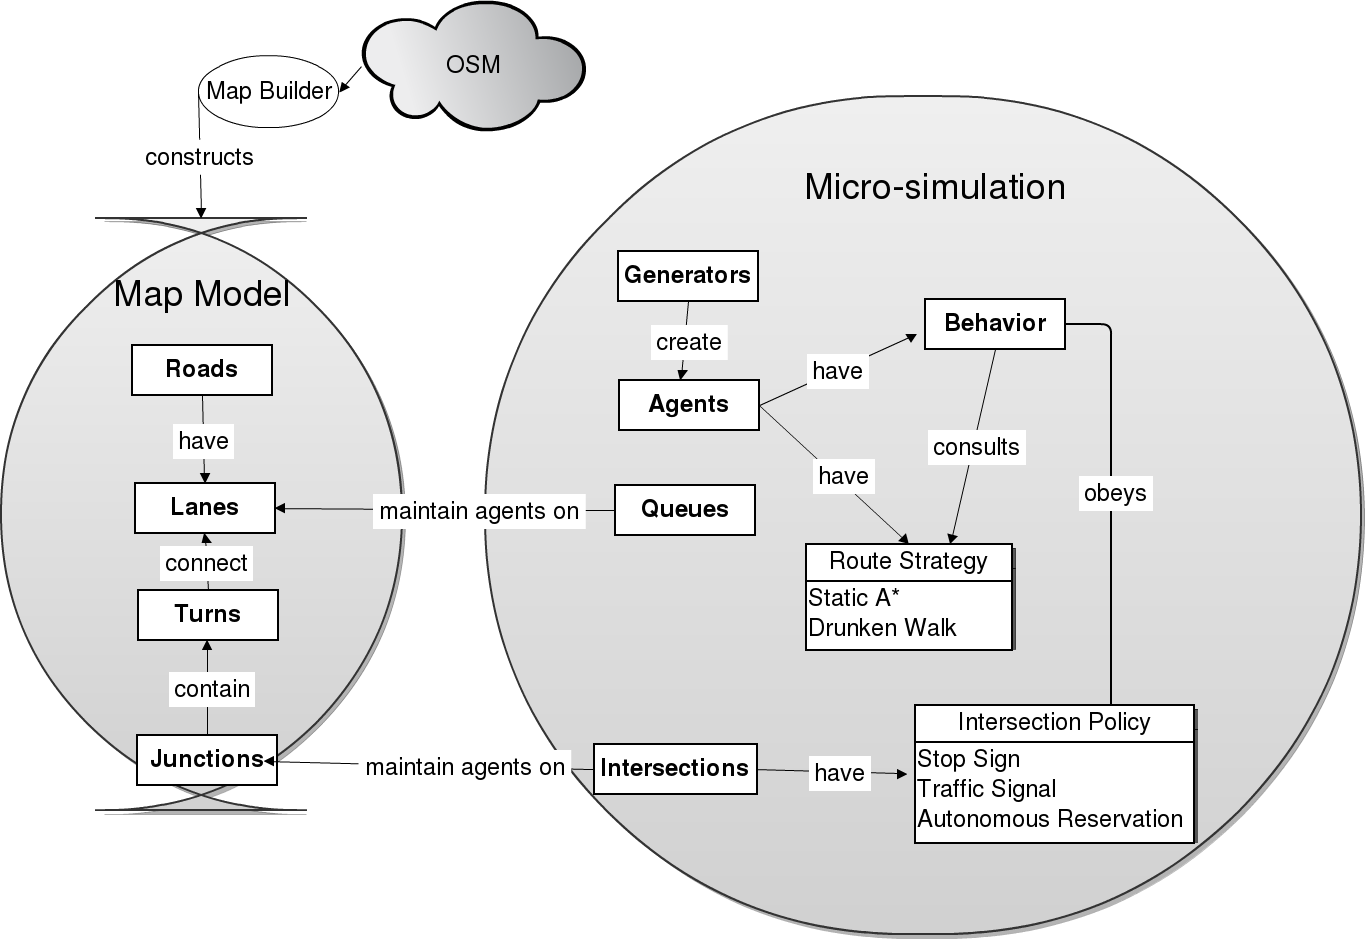
\includegraphics[scale=0.3]{architecture.eps}}
  \end{center}
}

The architecture and implementation notes of AORTA follow. AORTA is divided into
roughly three components, each somewhat independent of the others. The map model
handles everything from building graphs from OSM source to pathfinding. This
component is cleanly separated from the simulation engine, which adds the notion
of agents, structures on top of map components that detect collisions, and the
machinery to implement AORTA's model of car dynamics. If a future experiment
demands macrosimulation or cellular automata method, no changes to the map
infrastructure are needed, due to the software engineering. Finally, there is a
UI using Java Swing, which is (out of necessity) tied to both the map and
simulation components. The software has a documented API, is open-source, and
contains all of the code for the experiments described in Section 6 -- it is
designed for extensibility.

AORTA's implementation uses Scala, a language implemented on the Java Virtual
Machine. Scala provides the advantage of functional programming constructs while
still permitting imperative style. Parts of AORTA or extensions or clients can
just as easily be written in Java.

There are three standalone applications in AORTA. The map builder takes an OSM
file as input and produces an AORTA graph as output. There is a UI, using Swing,
to interactively explore the map and run simulations. Specific traffic patterns
can quickly be simulated by selecting a source and destination group of roads in
the UI. Finally, there is a headless mode that runs some specific experiment
without the overhead of visualization. The UI and headless mode both take a
graph as input, meaning the map construction step must be run once per OSM
input, but the same graph can be reused indefinitely.

%%%%%%%%%%%%%%%%%%%%%%%%%%%%%%%%%%%%%%%%%%%%%%%%%%%%%%%%%%%%%%%%%%%%%%%%%%%%%%%%

\section{MAP CONSTRUCTION FROM OSM}

Our goal is to simulate traffic on existing infrastructure, not contrived,
randomly generated maps. We do this by utilizing OpenStreetMaps, a community
project offering user-editable, free maps.  To run a simulation on a map from
OSM, there is a one-time conversion process to transform the map into AORTA's
format, which is also encoded with XML. It is split into 3 passes, each feeding
the next.

\subsection{Map Model}

\commentd{a simple diagram of a road with a few edges connected maybe to a
one-way}

\commentd{terminology is awkward. if we bold-face our notions of edge and vertex
every time we use them, would that better distinguish them from a graph's
verts/edges?}

\emph{Roads} are undirected edges between \emph{vertices}, which are
intersections between multiple roads. A \emph{road} contains one or two sets of
directed \emph{edges}, each of which represents a single lane of travel. One-way
\emph{roads} are supported. An \emph{edge} leads from one \emph{vertex} to
another; the second \emph{vertex} then contains a mapping from each incoming
\emph{edge} to some outgoing \emph{edge}; each pair is a \emph{turn}. Strictly
speaking and with confusing terminology, the multigraph consists of lanes
(\emph{edges}) as vertices and \emph{turns} as edges. \emph{Roads} are
super-structures with meta-data, bundling several \emph{edges} together, and
\emph{vertices} serve to bundle together \emph{turns}.

Geometrically, a road has a sequence of points defining the line segments
constituting the center yellow line. These points could also be interpreted as
control points for a curved road, but AORTA approximates using straight lines.
Edges mimic this geometry, projecting the center line some multiple of a lane's
width away in the appropriate direction. Turns are modeled with a single
straight line connecting the end of one edge to the start of another (so right
turns often have $0$ length). Since both edges and turns can support traffic,
they are grouped together as \emph{traversables}, meaning they have some
sequence of line segments and a total length.

\subsection{Pass 1}

The relevant parts of OSM's map model are nodes and ways. A node corresponds to
a GPS location, and ways are links between many nodes, corresponding to
driveable streets and other paths. The first pass reads OSM's XML format,
gathering ways as a series of coordinates. Ways implicitly intersect when a node
is used by multiple ways.

Since OSM also encodes pedestrian paths, bike routes, and even lakes with ways,
pass 1 filters out anything that does not seem to be driveable. OSM does not
seem to provide a unified list of valid roads, so these heuristics are
imperfect.

Finally, coordinates are normalized from GPS (longitude, latitude) to a
Cartesian coordinate system with no negative coordinates and the Y coordinate
increasing upwards. This is only done for convenience of manipulation in the UI.
Any coordinate is translated back to its original GPS form when used for
computing traversable length.

\subsection{Pass 2}

AORTA's structure demands a traditional definition of edge linking exactly two
vertices, rather than OSM's ways going through many common nodes. Pass 2 walks
along each way's coordinates, dividing it into multiple undirected edges.

\subsection{Pass 3}

Finally, pass 3 performs successive transformations to produce the final graph,
which is saved in XML.

\subsubsection{Making Lanes}

\commentd{the geometry was already explained in Map Model; I think it belongs
there if we have to cut one}

Undirected edges are first multiplied into directed lanes. The coordinates from
a slice of an OSM way are interpreted to be the center line of the road, and
lanes are placed by projecting the width of a lane perpendicularly from the
center line in either direction. OSM encodes one-way streets, so in this case,
if there are an odd number of one-way lanes, the middle lane is placed where the
center line would be, and the other lanes are shifted from there. If there are
an even number, then the middle two are both equidistant away from the invisible
center line. The number of lanes is guessed from OSM's annotation of the way's
``type.'' OSM's specification includes a tag for number of lanes, but in
practice as of the time of writing, it is rarely used.

\subsubsection{Making Turns}

Next, turns are constructed at each vertex between the incoming and outgoing
edges. This is completely heuristic based: we classify a potential turn as a
left, right, or straight turn based solely on angles between edges and if the
edge's original OSM ID matches. U-turns are constructed at dead-ends. If several
lanes all cross into fewer lanes, merging is forced for the rightmost lanes.
These patterns are attempts at generalizations; this process results in many
intersections having the incorrect turns. However, without a more detailed
source, this is the best compromise. At the time of writing, even sources like
Google Maps lack this information. (TODO how do you cite a lack of something?)
Finally, the geometry of a turn is simplified to a single line between the ends
of the edges it connects.  In the future, a more realistic curve could be drawn.

\commentd{illustration of turn conflicts}

AORTA has a low-granularity model of turn conflict. If two vehicles at any point
along two different turns could ever come into contact, then the turns are
always in conflict, no matter where the agent specifically is along that turn.
The alternative of tiling intersections (like \cite{JAIR08-dresner} does) would
provide more granularity, but it adds computational complexity and would be
impractical for many of the complex intersection geometries inferred from OSM.

\subsubsection{Ensuring connectivity}

Because turns are constructed imperfectly, most large graphs have edges that are
not reachable from some portions of the graph. Simulation and pathfinding would
suffer greatly if this remained the case, so pass 3 uses Tarjan's linear-time
algorithm for locating strongly connected components to remove the components of
the directed graph with the fewest members. (There is also a debugging switch to
leave these components in and highlight them in the UI.) The algorithm operates
at the granularity of lanes. If several lanes of many are disconnected within
one road, then the bad lanes are spliced out. This results in visually
unappealing geometric gaps, but if the entire road were removed, then Tarjan's
algorithm would have to be repeated to determine what edges the good lanes would
then disconnect. The end result is a connected digraph, ideal for corner
case-free pathfinding and simulation.

\subsubsection{Cleaning up geometry}

A road's center line correctly meets adjoining roads' center lines in the middle
of an intersection. Since the lines for a lane are parallel to the center line
and have the same length, they also meet in the intersection. This is
geometrically incorrect; lanes stop along the border of the intersection. Thus,
pass 3 includes heuristics to trim a lane's lines to the spot where they
intersect with another lane's lines. This results in a more accurate model, but
the process is imperfect, so sometimes lines extend too far or not far enough.

\subsubsection{Hierarchial divisions of the graph}

\commentd{i don't think this'll have much coverage in the rest of the paper; should
 we describe wards?}
\commentm{We aren't actually using wards at all yet.  I think we should save this
for a later paper.}

\subsection{Limitations}

\commentd{this maybe doesn't belong in this paper}

proposals to change OSM to fix these issues

projecting lines sucks... but all it really does is clutter UI
filtering out invalid ways in pass 1 is really not a clear process
number of lanes and speed limits... road types are wacky and wrong
turns are brittle.. detecting right-turn only lane is rare. shared center lane?
  not part of our model, or OSM's.
removing sccs is not ideal

\subsection{Integrating other data sources}

In the future, we intend to support the ability to augment an AORTA map with
data from non-OSM sources, such as information about the presence of extra lanes
for left turns. Using data such as GPS coordinates and road names, we could fuse
this extra information into an OSM-based AORTA map to make simulations on that map
that much more realistic.

Section 5.1 details a way to specify where traffic should originate and move
towards using the UI. This allows a more accurate simulation of situations such
as rush hour. In the future, we hope to be able to generate these demand
descriptions from government-collected data about a municipality's road usage.

%%%%%%%%%%%%%%%%%%%%%%%%%%%%%%%%%%%%%%%%%%%%%%%%%%%%%%%%%%%%%%%%%%%%%%%%%%%%%%%%

\section{SIMULATION}

AORTA uses microscopic simulation, modeling individual drivers as agents.
Discrete-time simulation is used, meaning an agent accelerates at a fixed rate
for the duration of a ``tick'' (also referred to as ``step'') to achieve a new
position and velocity. The tick duration $dt$ is configurable and fixed for the
simulation. Agents know this value and use it to reason about collision
avoidance and satisfying other constraints, so setting this value to the
average ``reaction time'' of a human driver may be appropriate. Each tick, the
simulation performs the following steps:

\begin{enumerate}
  \item Introducing new agents into the map
  \item Updating the position and velocity of agents
  \item Checking for collisions
  \item Allowing each agent to react
\end{enumerate}

Agents have few enforced constraints -- they cannot exceed their physical
acceleration capabilities, travel in reverse, or travel past the end of a
traversable without appearing on the next. Intersection policies and avoiding
collisions on the same traversable are the source of the other constraint in the
simulation, but it is the job of a behavior to satisfy those. There are three
main components of the simulation, each configurable by extending default
classes: agent behaviors, routing strategies, and intersection policies. Each
will be described below.

\commentd{justify arbitrary constants, like deaccel for cars;
          systems ideas, or limitations.. trylocks, atomic sim update, deadlock
          issues;
          limit: no lane-changing}

\subsection{Spawning}

To introduce new agents into the simulation in real-time, users create
\emph{generators} programatically or using the UI. A generator picks a random
starting position and random goal from two sets of roads chosen by the user. A
generator may cover the entire map, uniformly distributing traffic everywhere,
or it can mimic rush-hour scenarios. Every tick, a generator creates some number
of new agents.  If the agent's route policy needs work to be done (such as
pathfinding), the generator either performs it immediately (incurring a delay in
simulation if it is running) or sends it to a pool of worker threads to compute
in the background. When a generator finishes the work for an agent, it promotes
it to the ``ready'' state.

Once an agent's route is ready, the agent waits alongside its starting edge (as
if they are in a driveway or parking lot). At the beginning of each tick, they
enter with zero initial speed, if it is safe to do so. The list of agents
currently on the edge determines safety. Because behaviors must enforce speed
limit along an edge by the time an agent enters the road, then if there is no
agent within the worst-case distance (travel distance at the speed limit, plus
stopping distance from this speed) before the spawn point, then the new agent
may enter. To render unnecessary the prediction of which agents could enter the
edge in the near future, there is a buffer space at the beginning of the edge
where a new agent may never spawn. This disqualifies some short edges from being
spawn points, but this is not a troublesome issue in practice.

\subsection{Collision checking}

There are two structures to detect collisions. All traversables (edges and the
straight line-approximation of turns) maintain a \emph{queue} of occupying
agents, ordering them so that the agent farthest along is at the head of the
queue. A naive method of collision detection would detect an agent passing an
agent on the same queue, or entering a new queue not at the end, immediately
after an agent moves. However, agents take their steps sequentially and in an
effectively random order. Ideally they could be reordered so that agents in the
front of a queue always move first. Since the first agent may cross into the
next queue, that introduces a depdendency between traversables. A topological
sort of a directed graph containing circuits is not possible though, and since
we guarantee connectedness, there are necessarily circuits in maps.  Instead,
collisions are checked after every agent has stepped forward in time, treating
each time-step as atomic. Queues remember the original order of agents before a
step, and afterwards can verify that the order is still legal, with new agents
on the end and existing agents in the same order.

Likewise, intersections check for collisions after everybody has moved by
examining the turn each agent is performing and verifying that no other agent is
simultaneously performing a conflicting turn.

\subsection{Agent Reactions}

Each agent has a ``behavior'' governing it. When the agent travels past the end
of an edge during its step, the behavior picks the turn to pursue. Each tick,
the behavior can make the agent react by performing one of two actions:
disappearing from the map (only when the agent is at rest and is done with its
route) or setting an acceleration for the next step. In the future, another
possible action will be initiating a lane-change or merge.

Currently, the primary behavior used by all agents is the ``route-following
behavior.'' It is a generalized, baseline behavior that guarantees not to
collide with another agent or enter an intersection at the wrong time. Since it
picks the fastest conservative (safe) choice of acceleration at each step, it
could be easily extended to mimic human drivers by traveling at some random
amount less than this or to optimize fuel efficiency by tuning acceleration.

\subsubsection{Worst-case analysis and lookahead}

Since agents know the fixed $dt$ duration, they may reason about what could
happen during the next tick to avoid collision and illegal intersection entry.
The conservative analysis is to determine worst case -- how far could an agent
travel by the end of the next tick? If they accelerate as fast as possible for
$dt$, this gives them the longest possible traveling distance and highest
possible speed. Adding the stopping distance for this speed to the traveling
distance gives the worst-case distance.

\commentd{how much formula? pretty simple so far, but can certainly include them.
 should this part be worded like a proof? (because it can be)}

The worst-case distance may exceed the distance remaining on the agent's current
traversable. That means they could start or finish a turn during the next tick.
Because edges are often extremely short due to mis-marked ways in OSM (less than
$???$ meters), they may travel through several traversables during the next
move. Thus, any conservative behavior must look ahead until the worst-case
distance is exhausted, asking the route strategy which turn an agent will choose
in the future. At each traversable considered, there are 3 constraints to
satisfy: obeying the intersection, avoiding collision with another agent, and
obeying speed limits. Each constraint contributes to the max acceleration that
will obey the limit, so ultimately the result of lookahead will be the minimum
of these candidates.

Obeying a road's speed limit is a simple constraint. Like many parameters of the
map, speed limits are inferred from the road type claimed by the OSM source.

\subsubsection{Obeying intersections}

A behavior's interaction with an intersection policy amounts to polling it with
the turn the agent wants to perform, the distance away the agent currently is,
and how long the agent has been waiting (so policies can enforce a required
delay before entering the intersection). The intersection policy simply orders
the agent to ``stop'' or ``continue.'' The lookahead considers no intersections
beyond the first that issues ``stop'', since the behavior cannot legally proceed
past that one anyway. The acceleration to avoid entering an intersection
attempts to end a configurable threshold back from the end of a traversable to
account for crosswalks and as an epsilon value, since achieveing a distance
along an edge equal to its length means spilling over into the next traversable,
which the intersection has banned. Sometimes stopping behind this threshold is
not possible -- namely, when the edge length is shorter -- and in that case,
anywhere before the end is acceptable.

\commentd{include some form of piyush's proof about accel to end?}

\subsubsection{Optimal tailgating}

\commentd{diagram with overlapping distances}

When the lookahead analysis is considering some future traversable, it only has
to consider the agent closest to the start of it in the present. An edge may
only be entered from a turn, so the intersection policy has the burden of
ensuring no agent performs a turn that leads to the same edge simultaneously.
Following an agent safely means maintaining a configurable following distance
behind the agent. Worst-case analysis is again used: the most dangerous move the
agent in front could perform is decelerating as fast as possible the next tick,
and the worst-case traveling distance for the agent following is already known
from lookahead (speeding up as much as possible).

Maintaining following distance from agents actually enables a form of deadlock
in the simulation. If an agent is forced to stop in an intersection mid-turn due
to its destination edge filling up with other agents, then nobody may cross the
blocked intersection. With many agents in a small area, this situation may
occur several times in an interdependent way. The solution currently being
investigated will require behaviors to ensure a turn may be fully completed
before starting it. This will prevent intersections from ever being blocked.

\commentd{diagram showing deadlock, or lookahead in gen eral}
\commentd{i really hope to fix this issue soon, but it's not an immediately easy
fix}

\subsection{Routing Strategies}

Picking accelerations that optimize some objective functions is a separate task
from picking a path to travel. Thus, the behavior described above can consult
any route strategy. Currently two simple implementations are available. One
statically plans a route to some goal using standard the A* search; the other
performs a drunken walk, lazily planning random choices at each intersection as
the lookahead engine needs to know. Future experiments in dynamic replanning or
hierarchial planning can be performed without modifying any code other than a
creating new route implementation. Route policies could also interact with a
singleton overseer to have some sort of global insight.

\subsection{Intersection Policies}

Agents and behaviors (on behalf of an agent) poll an intersection as they
approach it, asking if they should stop or not. A policy is free to prevent
agents from performing conflicting turns concurrently by any means. Two main
policies exist already, but implementing the interface for extensions is simple.

The stop sign policy works by maintaining a current owner and a queue of waiting
agents. An agent can enter the queue only when they are within some threshold of
the start of their turn (a constraint satisfied by the default lookahead
behavior), even if that is several (rather short) edges and turns away. After
the head of the queue has waited for a configurable pause, they obtain the lock
and have exclusive access to the intersection, releasing it only when they
complete their turn.

A form of deadlock is possible in a sequence of short edges and turns. Agent
$A_1$ acquires the lock to intersection $V_1$, but needs the lock to $V_2$ to
proceed. Meanwhile, $A_2$ has the lock for $V_2$ and needs the lock for $V_1$.
To deal with this circumstance, an agent's behavior can yield any held locks (a
notion generalized to any intersection policy) when its speed is $0$ and its
conservative acceleration is to remain at rest. The stop sign policy only
removes an agent's lock if it has not started its turn (because otherwise, the
agent is stalling in the intersection). The next time that agent polls, the
policy restores the agent to the front of the queue.

\commentd{hopefully we'll have a neater solution than the above soon}

\commentd{describe traffic signal policy, once it's working}

Intersection policies are one of the most intriguing piece of the simulation to
tweak. Future policies will include stop lights that adaptively learn better
timings and an AIM-esque reservation system \cite{JAIR08-dresner}.

\subsection{Determinism and other simulation properties}

AORTA is designed for controlled experiments. Consequently, simulations are
deterministically reproducible. A single seed for the pseudo-random number
generator, the input graph, and the generators' configuration completely
determine the outcome of any simulation. This determinism does break down when
generators use worker threads, since routes may be computed in different orders,
causing agents to be ready to enter the road at different times.

\commentd{saving a ``scenario'' can soon be a feature}

\commentd{and how will we solve this issue with threads and determinism?}

\commentd{give some informal or formal (with numbers) idea of scale / how many
agents we can simulate in different map sizes}

%%%%%%%%%%%%%%%%%%%%%%%%%%%%%%%%%%%%%%%%%%%%%%%%%%%%%%%%%%%%%%%%%%%%%%%%%%%%%%%%

\section{EXPERIMENTAL RESULTS}

\commentd{upgrading stop signs to signals, optimizing timing?}

%%%%%%%%%%%%%%%%%%%%%%%%%%%%%%%%%%%%%%%%%%%%%%%%%%%%%%%%%%%%%%%%%%%%%%%%%%%%%%%%

\section{CONCLUSIONS}

Write me. big future ideas:

contraflow

microtolling

dynamic replanning

autonomous intersections

\addtolength{\textheight}{-12cm}  % This command serves to balance the column lengths
                                  % on the last page of the document manually. It shortens
                                  % the textheight of the last page by a suitable amount.
                                  % This command does not take effect until the next page
                                  % so it should come on the page before the last. Make
                                  % sure that you do not shorten the textheight too much.

%%%%%%%%%%%%%%%%%%%%%%%%%%%%%%%%%%%%%%%%%%%%%%%%%%%%%%%%%%%%%%%%%%%%%%%%%%%%%%%%

\section*{APPENDIX}

Probably stuff about getting and using the code.

\section*{ACKNOWLEDGMENT}

Dr. Quinlan has certainly been helpful.

What credits do we need to give to OSM?

%%%%%%%%%%%%%%%%%%%%%%%%%%%%%%%%%%%%%%%%%%%%%%%%%%%%%%%%%%%%%%%%%%%%%%%%%%%%%%%%

% Notes.

%possible background/links

%http://www.caliper.com/transmodeler/default.htm
%http://ieeexplore.ieee.org/stamp/stamp.jsp?tp=&arnumber=6082793
%https://www.google.com/search?sourceid=chrome&ie=UTF-8&q=Agent-Based+Traffic+Simulation+and+Traffic+Signal+Timing+Optimization+with+GPU

%%%%%%%%%%%%%%%%%%%%%%%%%%%%%%%%%%%%%%%%%%%%%%%%%%%%%%%%%%%%%%%%%%%%%%%%%%%%%%%%

\bibliographystyle{IEEEtran}
\bibliography{root}

\end{document}
